
\documentclass{article} % For LaTeX2e
\usepackage{iclr2026_conference,times}

% Optional math commands from https://github.com/goodfeli/dlbook_notation.
\input{math_commands.tex}

\usepackage{hyperref}
\usepackage{url}
\usepackage{amsmath}
\usepackage{amssymb}
\usepackage{booktabs}
\usepackage{tikz}
\usetikzlibrary{arrows.meta,positioning,shapes.geometric,fit,backgrounds}
\usepackage{graphicx}
\title{CatanAgents: Long-Term Planning Agents for Playing Settlers of Catan}

% Authors must not appear in the submitted version. They should be hidden
% as long as the \iclrfinalcopy macro remains commented out below.
% Non-anonymous submissions will be rejected without review.
\author{
Dhruv Malpani \quad
Rudy Juarez-Ovallos \quad
Sharayu Janga \quad
Vayun Gupta \\
University of Illinois Urbana-Champaign \\
}

\iclrfinalcopy
\begin{document}


\maketitle
\lhead{}
\thispagestyle{fancy}

\section{Introduction}

Large language models show strong performance on reasoning and tool-use tasks, but their reliability in long-horizon, multi-step strategic environments remains unclear. Settlers of Catan is a useful stress test: strong play requires planning under uncertainty, partial observability, stochastic dice outcomes, changing board geometry, and multi-agent negotiation. Winning is not a matter of one good move---agents must balance expansion, hand efficiency, opponent blocking, development-card timing, and trade policy across many turns. Our companion benchmark argues that outcome-only evaluation is especially weak here, since a strategically sound move can still lose to dice variance while a brittle sequence can win if not punished.

Existing agents are insufficient in this setting for two reasons. First, single-stream ReAct-style agents overload one prompt with parsing full state, long-term planning, threat detection, negotiation, and legal action selection; in our early prototypes this produced hallucinated actions, lost context, weak opponent modeling, and high latency. Second, raw environment state is too noisy for stable decision making in a socket-driven multiplayer game that must also respond to asynchronous trade offers. Prior work reinforces this: LLMs remain brittle in strategic games requiring adaptation and consistency \citep{yao2022react,vidler2025playing}.

We propose a role-specialized multi-agent Catan system with four cooperating agents---\textbf{Strategy}, \textbf{Development}, \textbf{Trading}, and \textbf{Risk}---coordinated through a shared scratchpad. Strategy is the orchestrator: it updates shared state, invokes Risk for deterministic probability analysis and threat summaries, produces a turn-level plan, and delegates build, discard, robber, and trade decisions. Unlike generic multi-agent chat, communication follows an explicit code-enforced topology, each agent has a restricted tool subset, and Risk combines exact game math with a lightweight LLM narrative rather than free-form language reasoning. The design is intended to reduce prompt overload, improve legality, and persist strategic intent across turns \citep{belle2025agentsofchange}.

\section{Related Work}
\label{sec:related}

Our primary baseline is a \textbf{ReAct} Agent, which interleaves reasoning and action so a single LLM can plan while interacting with an environment \citep{yao2022react}. We depart from ReAct by decomposing decision making across specialized roles and constraining tool access per role, which reduces illegal actions and makes failures easier to trace. More broadly, our design is related to multi-agent LLM frameworks such as \textbf{CAMEL} and \textbf{AutoGen}, which use role specialization and inter-agent communication for complex tasks \citep{li2023camel,wu2023autogen}. Unlike those general-purpose systems, our architecture is domain-specific: each agent has a fixed Catan role and communicates through a typed, scratchpad-mediated, topology-restricted protocol. \textbf{Voyager} motivates persistent intermediate structure for long-horizon tasks \citep{wang2023voyager}; we adopt a tightly scoped variant that stores strategic state, trade context, and risk summaries rather than executable skills. The closest domain work is \textbf{Agents of Change} \citep{belle2025agentsofchange}, which studies self-evolving LLM agents for Catan; we instead target reliable in-game coordination and benchmarked decision quality during live play, complementing rather than replacing that line of work. Recent evidence that LLMs remain brittle in strategic games \citep{vidler2025playing} further motivates our hybrid math-plus-LLM design.

\section{Agent Design}
\label{sec:design}

\subsection{Architecture Overview}
\label{sec:arch}

CatanAgents is a decentralized cooperative system of four specialized LLM agents: the \textbf{Strategy} orchestrator and the \textbf{Risk}, \textbf{Development}, and \textbf{Trading} executors. All persistent state flows through a thread-safe \emph{Scratchpad}, and inter-agent control flow is restricted to the topology in Figure~\ref{fig:arch}, enforced at runtime by an \texttt{ALLOWED\_CHANNELS} whitelist in \texttt{BaseAgent}. Per turn, Strategy polls the socket, writes state to the Scratchpad, invokes Risk for deterministic probability analysis, asks GPT-4o for a structured plan, and delegates tactical phases to Trading and Development.

\begin{figure}[t]
\centering
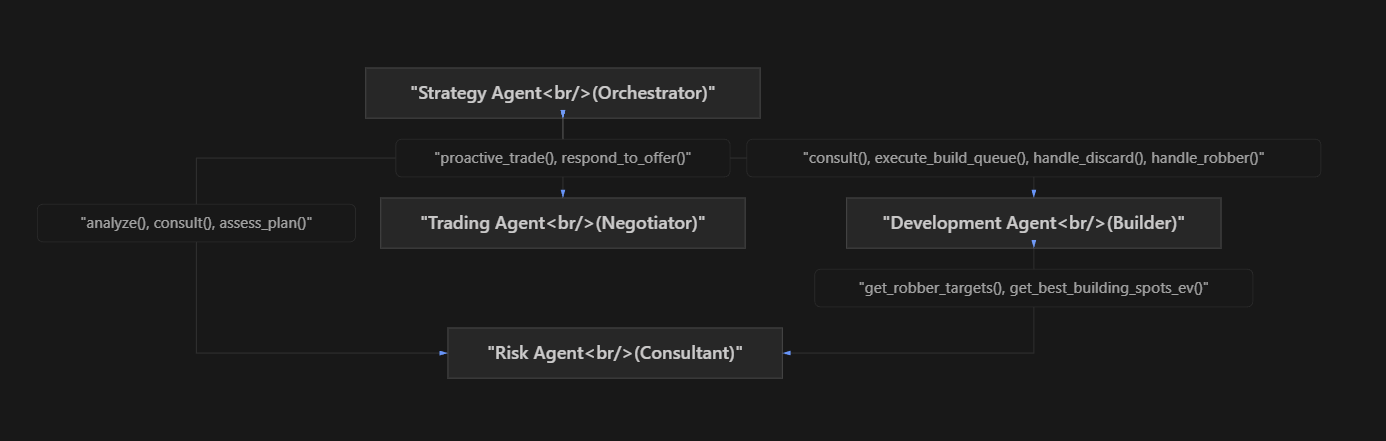
\includegraphics[width=0.95\linewidth]{Agent-graph.png}
\caption{Communication topology. Edges are the only allowed channels; \texttt{BaseAgent} raises \texttt{PermissionError} on any unauthorized call. Trading is isolated so all strategic input flows through Strategy's \texttt{TradePolicy}.}
\label{fig:arch}
\end{figure}

Five principles govern the design: (1) \emph{separation of concerns}, each agent owns one cognitive domain; (2) \emph{hierarchical coordination}, Strategy drives a typed control loop; (3) \emph{hybrid reasoning}, deterministic math for probability-critical quantities and LLMs only for ambiguous decisions; (4) \emph{graceful degradation}, every LLM call has a deterministic fallback; and (5) \emph{thread safety}, a single \texttt{threading.Lock} on the Scratchpad serializes the background socket listener and the main agent loop.

\subsection{Shared Infrastructure}
\label{sec:shared}

\paragraph{Scratchpad:} The Scratchpad is the only mechanism for cross-agent state. It exposes nine regions, written with typed Python dataclasses rather than free-form dicts. \texttt{game\_state}, \texttt{processed\_state}, and \texttt{state\_json} hold raw, structured, and LLM-optimized views of the game (all written by Strategy). \texttt{risk\_analysis} (Risk) stores a \texttt{RiskAnalysis} with expected income, threat rankings, robber EVs, and a narrative. \texttt{strategy\_plan} (Strategy) holds a \texttt{StrategyPlan} with goals, build queue, and \texttt{TradePolicy}. \texttt{trade\_state} (Trading) tracks per-opponent reputation, pending offers, and trade history. \texttt{build\_log} (Development) and \texttt{action\_log} (all) are append-only audit trails; \texttt{inter\_agent\_messages} is a typed message queue. Because every region is a dataclass, turns are deterministically replayable from the logs.

\paragraph{Tool registry:} A unified \texttt{ToolRegistry} exposes 22 game actions and queries. Each tool carries (i) an OpenAI JSON schema used directly for GPT-4o function-calling, (ii) a phase filter (\texttt{roll}, \texttt{main}, \texttt{discard}, \texttt{robber}, \texttt{setup}, \texttt{specialBuild}), and (iii) an agent filter. Role-scoping is strict: \texttt{move\_robber} is Development-only; \texttt{bank\_trade}, \texttt{propose\_trade}, \texttt{respond\_to\_trade} are Trading-only. The registry computes the visible subset at prompt-construction time, dropping roughly half the tool descriptors from every agent-specific context.

\subsection{Per-Agent Design}
\label{sec:agents}

\textbf{Strategy} owns the game loop, polling state every 150--250\,ms and calling \texttt{risk.analyze()} and \texttt{risk.consult(question)} each turn. It builds a GPT-4o prompt from the \texttt{state\_json}, the \texttt{RiskAnalysis}, the Risk consultant's answer, the previous plan, recent messages, and ranked building spots, receiving back a \texttt{StrategyPlan} JSON with \texttt{long\_term\_goal}, \texttt{short\_term\_goals}, \texttt{priority\_resources}, \texttt{build\_queue}, \texttt{trade\_policy}, \texttt{should\_trade\_first}, \texttt{risk\_tolerance}, and \texttt{reasoning}. It then delegates by phase: main runs \texttt{trading.proactive\_trade()} then \texttt{development.execute\_build\_queue()}; discard and robber are forwarded to Development; off-turn, Strategy watches for incoming offers and wakes \texttt{trading.respond\_to\_offer()}. \textbf{Risk} is an interactive consultant with three modes---\texttt{analyze()} (runs the math in Section~\ref{sec:probs} plus a GPT-4o narrative), \texttt{consult(question)} (answers a turn-relevant question selected from a small decision table), and \texttt{assess\_plan(plan)} (critiques a draft plan)---all with deterministic template fallbacks.

\textbf{Development} executes \texttt{StrategyPlan.build\_queue} in priority order via registry tools; failures are skipped and logged rather than re-planned, because the server is the authority on legality. For \emph{discard} on 7-rolls, GPT-4o selects cards via \texttt{discard\_cards} using Strategy's \texttt{priority\_resources} (up to two repair rounds, then a greedy non-priority fallback). For \emph{robber}, Development calls \texttt{risk.get\_robber\_targets()} for hexes ranked by net damage, optionally lets GPT-4o override, and falls back to an adjacency-count heuristic. \textbf{Trading} runs in two modes: \emph{proactive} (our turn) runs a 6-step ReAct loop over trading tools (\texttt{bank\_trade}, \texttt{propose\_trade}, \texttt{counter\_trade}, \texttt{cancel\_trade}, \texttt{get\_trade\_options}, \texttt{get\_trade\_offer\_status}), falling back to a bank trade then a 1-for-1 proposal; \emph{reactive} (off-turn) deduplicates incoming offers by signature hash and runs a 2-step loop restricted to \texttt{respond\_to\_trade}/\texttt{counter\_trade}, falling back to the deterministic score in Section~\ref{sec:probs}. A per-opponent reputation in $[-1,1]$ ($+0.05$ per accept, $-0.03$ per decline) biases proposal targeting; opponents at $\geq 8$ VP are blocked from proposals entirely.

\subsection{Token-Efficient State Summary}
\label{sec:summary}

Raw \texttt{getPlayerView} contains hundreds of hex, vertex, and edge entries that would dominate an LLM prompt. The Scratchpad emits a compact summary via \texttt{to\_state\_json()} with seven regions---\texttt{meta} (phase, turn, dice), \texttt{scoreboard} (VP, per-opponent cards/knights/road length), \texttt{my\_state} (resources, dev cards, pieces left, trade ratios, buildings), \texttt{board\_signals} (robber hex, longest road, largest army), \texttt{risk\_summary} (expected income, top threat, narrative), \texttt{active\_trade}, and \texttt{recent\_delta}---which every agent prompt consumes. The summary gives consistency across agents on a given turn and is roughly $10\times$ smaller than the raw payload, keeping multi-step ReAct loops within the GPT-4o context budget.

\subsection{Probability and Decision Model}
\label{sec:probs}

Probability-sensitive decisions are handled by deterministic heuristics rather than free-form LLM reasoning. We estimate expected production from adjacent hex probabilities (with city/settlement multipliers and robber blocking), compute opponent threat using a weighted score over victory points, income, cards, and achievement proximity, and rank candidate settlement/city actions with scarcity-aware resource weights. Trading decisions use a bounded heuristic score with threshold-based accept/counter behavior, and an approximate win-probability signal is derived from victory points, income, development progress, and proximity to key achievements. This deterministic layer provides stable, auditable signals that are then summarized for the planning agents.

\section{Experimental Setup}
\label{sec:setup}

\paragraph{Benchmark:} We evaluate on \textbf{CatanBench}, our companion benchmark for strategic reasoning in Settlers of Catan. It contains 20 tasks spanning short-term tactical choices, medium-horizon resource and build prioritization, and long-term strategic commitments, and it scores the \emph{quality} of decisions during live play rather than final game outcomes alone. The benchmark is described fully in our benchmark paper; we summarize only the parts relevant to agent evaluation.

\paragraph{Baselines:} We compare against two systems. \emph{Single-Prompt ReAct}: one LLM with the full tool interface handles all reasoning and action execution alone---the most direct test of whether role specialization improves over a standard tool-using design. \emph{Rule-Based LLM}: the same environment interface but guided by hand-crafted Catan heuristics, providing a lower-structure baseline.

\paragraph{Metrics:} Gameplay metrics are win rate, average final victory points, and average rounds to win; reasoning metrics are task success rate and average task score across the 20 tasks; operational metrics are average per-turn latency, illegal-move rate, and retry rate. Overall performance is summarized with a weighted aggregate over normalized win rate, VP, rounds-to-win, task score, and latency; we report means, standard deviations, and confidence intervals across trials.

\paragraph{Protocol:} All agents run under identical seeds and environment settings. We plan approximately \textbf{20--30 full-game trials} per system plus the full benchmark task set, across varied seat positions and map configurations. Each run logs structured traces of state transitions, chosen actions, legality, latency, token usage, API cost, and benchmark scores. Because full-game evaluation is still running at submission time, the final version will report exact model versions and trial counts.

\section{Results}
\label{sec:results}

We evaluated three agents across pairwise Catan games: a single-agent ReAct baseline, a rule-based heuristic baseline, and our multi-agent Strategy system. Table~\ref{tab:results} reports aggregated results across the completed comparisons. ReAct achieved the strongest game outcomes, winning its matchups against both Strategy and the heuristic baseline. The heuristic agent had the strongest execution reliability and lowest latency, while Strategy was faster than ReAct but struggled to convert plans into victory points.

\begin{table}[h]
\caption{Aggregated headline comparison across completed head-to-head evaluations.}
\label{tab:results}
\begin{center}
\small
\begin{tabular}{@{}lcccc@{}}
\toprule
\textbf{Agent} & \textbf{Win rate} & \textbf{Avg VP} & \textbf{Task score} & \textbf{Latency} \\
\midrule
ReAct Agent       & 100.0\% & 10.0 & 0.783 & 9954 ms \\
Rule-Based Heuristic      & 50.0\%  & 9.0  & 0.663 & 3236 ms \\
Strategy Agent        & 0.0\%   & 5.0  & 0.623 & 5710 ms \\
\bottomrule
\end{tabular}
\end{center}
\end{table}

Performance also varied by task horizon. Strategy performed best on short-term tasks against ReAct, completing $64.2\%$ compared to ReAct's $50.0\%$, showing that the multi-agent planner helps with structured immediate decisions. However, ReAct performed better on medium- and long-term tasks, reaching $86.4\%$ and $86.7\%$, while Strategy reached $80.8\%$ and $60.0\%$. Against the heuristic baseline, both LLM agents were less reliable on short-term execution, where the heuristic agent consistently achieved near-perfect task completion.

Qualitatively, ReAct excelled in dynamic board states by using city upgrades, robber moves, and Longest Road to convert position into wins. Strategy showed coherent planning behavior, but sometimes failed to translate those plans into legal or high-value actions. These results suggest that structured planning improves speed and short-term consistency, while adaptive reasoning is more effective for long-term gameplay decisions.

\section{Discussion}
\label{sec:discussion}

\paragraph{What works.} Role-scoped tool sets substantially reduce the prompt surface each agent sees and in early testing eliminated a class of illegal actions seen with the single-ReAct prototype (e.g., Trading attempting \texttt{move\_robber}, or Development proposing trades out of phase). Typed Scratchpad dataclasses make plans and risk analyses inspectable turn-by-turn, and because every LLM call has a deterministic fallback, the system has never stalled when OpenAI is unavailable---it runs on heuristics and logs the degradation. The \texttt{state\_json} summary keeps prompts consistent and short enough that multi-step ReAct loops stay within context without truncation.

\paragraph{What does not work yet and limitations.} The largest gap is Development's end-to-end build-queue executor, which reliably handles discard and robber but still fails on a subset of city-upgrade and road-building items---the current blocker for full-game evaluation. Strategy's LLM-generated queues occasionally reference vertex keys that opponents claim before execution; skip-and-continue hides this from the server but wastes queue slots. Proactive ReAct trading is also expensive: a 6-step GPT-4o loop can dominate per-turn cost while often matching the deterministic heuristic, suggesting the LLM should be invoked only when the heuristic is uncertain. The design assumes standard 4-player Catan and does not model expansions or cross-game self-improvement in the style of \citet{wang2023voyager} or \citet{belle2025agentsofchange}. GPT-4o cost per full game is nontrivial; our fallbacks are deliberately structured to make swapping in a smaller local model mechanical.

\section{Conclusion}
\label{sec:conclusion}

We have described CatanAgents, a role-specialized four-agent LLM system for Settlers of Catan that combines deterministic probability analysis with LLM-driven planning through a typed shared Scratchpad and a strict, code-enforced communication topology. The design contributes a concrete blueprint for decomposing a long-horizon strategic game across LLM agents while keeping probability-critical decisions exact and making strategic intent persistent across turns. Immediate future work is to complete the Development executor and run the full CatanBench evaluation; longer-term, we plan to add a cross-game self-improvement loop over the action log, swap in smaller local models behind the existing heuristic fallbacks, and extend the framework to Catan variants and larger player counts.

\begin{thebibliography}{99}

\bibitem[Belle et~al.(2025)]{belle2025agentsofchange}
Nikolas Belle, Dakota Barnes, Alfonso Amayuelas, Ivan Bercovich, Xin Eric Wang, and William Wang.
Agents of Change: Self-Evolving LLM Agents for Strategic Planning.
\textit{arXiv preprint arXiv:2506.04651}, 2025.

\bibitem[Li et~al.(2023)]{li2023camel}
Guohao Li, Hasan Abed Al Kader Hammoud, Hani Itani, Dmitrii Khizbullin, and Bernard Ghanem.
CAMEL: Communicative Agents for ``Mind'' Exploration of Large Language Model Society.
\textit{Advances in Neural Information Processing Systems}, 2023.

\bibitem[Vidler and Walsh(2025)]{vidler2025playing}
Alicia Vidler and Toby Walsh.
Playing Games with Large Language Models: Randomness and Strategy.
\textit{arXiv preprint arXiv:2503.02582}, 2025.

\bibitem[Wang et~al.(2023)]{wang2023voyager}
Guanzhi Wang, Yuqi Xie, Yunfan Jiang, Ajay Mandlekar, Chaowei Xiao, Yuke Zhu, Linxi Fan, and Anima Anandkumar.
Voyager: An Open-Ended Embodied Agent with Large Language Models.
\textit{arXiv preprint arXiv:2305.16291}, 2023.

\bibitem[Wu et~al.(2023)]{wu2023autogen}
Qingyun Wu, Gagan Bansal, Jieyu Zhang, Yiran Wu, Beibin Li, Erkang Zhu, Li Jiang, Xiaoyun Zhang, Shaokun Zhang, Jiale Liu, Ahmed Hassan Awadallah, Ryen W. White, Doug Burger, and Chi Wang.
AutoGen: Enabling Next-Gen LLM Applications via Multi-Agent Conversation.
\textit{arXiv preprint arXiv:2308.08155}, 2023.

\bibitem[Yao et~al.(2022)]{yao2022react}
Shunyu Yao, Jeffrey Zhao, Dian Yu, Nan Du, Izhak Shafran, Karthik Narasimhan, and Yuan Cao.
ReAct: Synergizing Reasoning and Acting in Language Models.
\textit{arXiv preprint arXiv:2210.03629}, 2022.

\end{thebibliography}

\end{document}
